\documentclass[11pt, oneside]{article}   	% use "amsart" instead of "article" for AMSLaTeX format
\usepackage{geometry}                		% See geometry.pdf to learn the layout options. There are lots.
\geometry{letterpaper}                   		% ... or a4paper or a5paper or ... 
%\geometry{landscape}                		% Activate for for rotated page geometry
%\usepackage[parfill]{parskip}    		% Activate to begin paragraphs with an empty line rather than an indent
\usepackage{graphicx}				% Use pdf, png, jpg, or eps§ with pdflatex; use eps in DVI mode
								% TeX will automatically convert eps --> pdf in pdflatex		
\usepackage{listings}
\usepackage{amssymb}
\usepackage{amsmath}
\usepackage{subfigure}

\lstset{language=Java, basicstyle=\scriptsize}


\title{CS675 Project 1: P2P Architecture}
\author{Zhonghua Xi}
%\date{}							% Activate to display a given date or no date

\begin{document}
\maketitle

\section{Design}
\subsection{Peer}
A peer node is both a client and server which provides both CAN service and bootstrap service.

\subsection{Routing}
When the coordinate of a target point $p$ is given, the CAN system routes the message in the following manner.
If current peer $P$'s zones contain $p$, $P$ processes the request. Otherwise $P$ forwards the request to its neighbor who is closest to $p$. The distance $D$ between a node $N$ and a point $p$ is defined as: 
\begin{equation}
D(N,p) = 
\begin{cases}
    0, 										& \text{if } N \text{'s zones contain } p \\
 	\min\limits_{i}(\lVert N.zone_i.center - p \rVert),      & \text{otherwise}
\end{cases}
\end{equation}
The above distance metic guarantees the message will be routed to the node whose zones contain $p$.


\section{Implementation}

\subsection{Language}
Java is chosen to implement this project since Java provides a lot of tools to deal with network communications.

\subsection{Networking Technique}
Java RMI is chosen as the networking technique. RMI can be regarded as an object-oriented version RPC which provides high level abstraction and low level of complexity.
Request and response become function parameters and returned value. 
The client will be blocked (by default) until receives the response. 
Compare to a socket based implementation, in which request and response are not deeply-related, the client code in RMI is more semantically meaningful and more elegant.

\subsection{Peer}
When a peer is about to start, a bootstrap server (ip/hostname and name) must be provided. Otherwise, that peer will think it is the only node in CAN and will occupy the entire zone.
The peer will provide both CAN service (join, insert, search) and Bootstrap (get active node list). These two services are bind to different names.

\subsubsection{Bootstrap Service}
For a peer as a bootstrap server, it has only one remote method as follow. This method will return randomly picked neighbors' peer\_ids/ips and itself's up to MAX\_NODES nodes (3 in current code).

\begin{lstlisting}
Map<String, String> getNodeList(String peerId, String ip)
      throws RemoteException;
\end{lstlisting}

\subsubsection{CAN Service}
For a peer as a CAN node, it is also a CAN server which provides CAN service (insert, search, join).
As mentioned in previous section, all requests that can not be handled by current peer will be forwarded to a closer peer recursively until reached a peer who can handle the request.
Let us take a look at the implementation search, other methods will be very similar in structure.

\begin{lstlisting}
public SearchResult searchCAN(String key) throws RemoteException {
    Point point = HashUtil.getCoordinate(key);
    SearchResult result = null;
    if (this.containsPoint(point)) {
      // if the target point in current zone, handle request
      List<String> files = this.getFiles(key);
      result = new SearchResult(this.peerId, this.ip, key, files);
    } else {      
      Node n = this.getNearestNeighbor(point);    // find the closest neighbor
      result = n.searchCAN(key);                  // forward the request
      result.prependRoute(this.peerId, this.ip);  // update the routing table    
    }
    return result;
  }
\end{lstlisting}

\subsection{Leaving Protocol}
When a node leaves CAN, it must migrate its zone to one of its neighbor. One way to migrate a zone is merging. The zone from the leaving node is merged into its neighbor's zone when they are mergeable, he merged zone should still be rectangle or square. However, in some cases, the leaving zone can not be merged to any neighbors. In this case, a node must be volunteered to store the zone temporarily and wait a new node to occupy the entire temp zone. However, if that nodes also leaves CAN, both its main zone and temp zones must be migrated to it neighbor and so on. This leaving protocol could lead to fragmentation. In this implementation, temp zones merging and self-merging are introduced to minimize fragmentation which will be detailed in the following section.

\subsubsection{Self-Merging}
When a node receives a temp zone, it will try to merge the temp zone with its main zone first, followed by temp zone / temp zone merging. If any of two zones were merged, this process is repeated, until none of two zones (either main zone or temp zones) owned by current node can not be merged anymore. An end to end scenario is shown in Fig.~\ref{fig:merging} and the screenshots of peer2's info before and after peer3 left is shown in Fig.~\ref{fig:screenshot}.

\begin{figure}[htbp] %  figure placement: here, top, bottom, or page
   \centering
   \subfigure[peer1 joined]{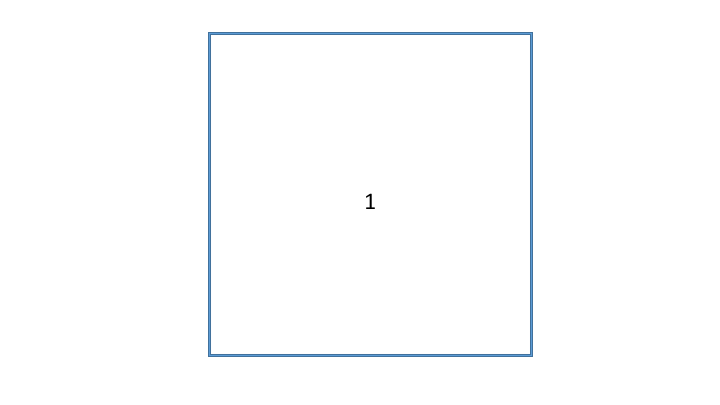
\includegraphics[width=1.5in, clip=true, trim=80mm 0mm 80mm 0mm]{figures/zone/Slide1.png}}
   \subfigure[peer2 joined]{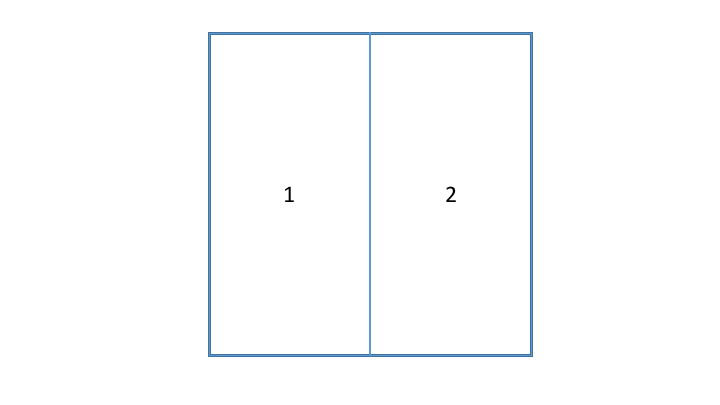
\includegraphics[width=1.5in, clip=true, trim=80mm 0mm 80mm 0mm]{figures/zone/Slide2.png}}
   \subfigure[peer3 joined]{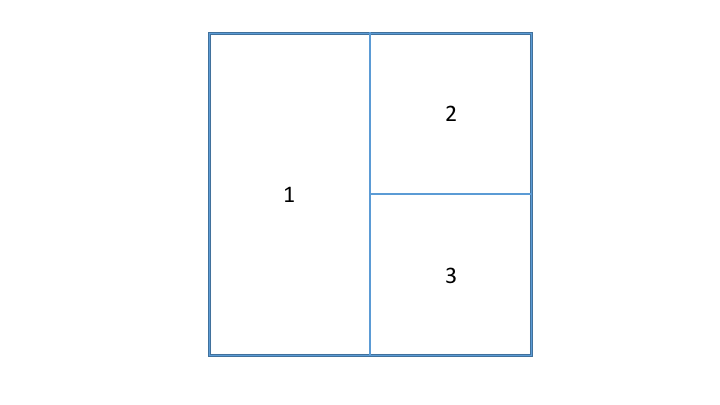
\includegraphics[width=1.5in, clip=true, trim=80mm 0mm 80mm 0mm]{figures/zone/Slide3.png}}
   \subfigure[peer1 left]{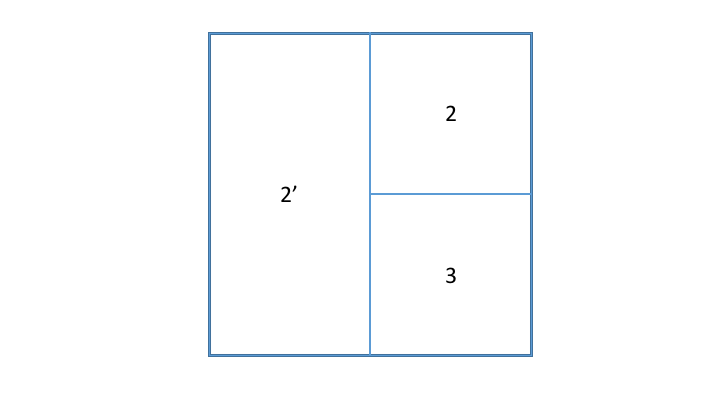
\includegraphics[width=1.5in, clip=true, trim=80mm 0mm 80mm 0mm]{figures/zone/Slide4.png}}
   \subfigure[peer3 left, before self merging]{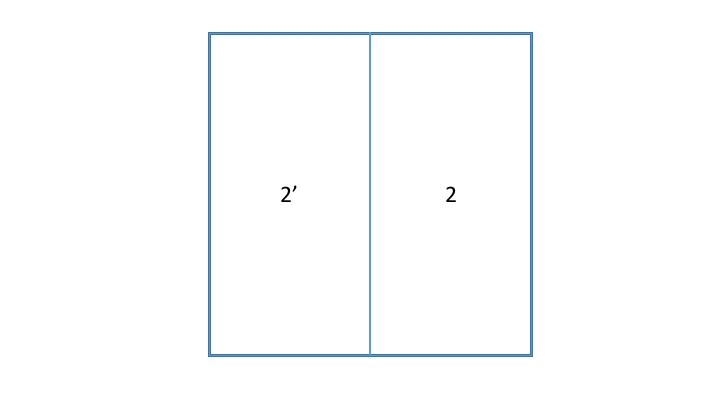
\includegraphics[width=1.5in, clip=true, trim=80mm 0mm 80mm 0mm]{figures/zone/Slide5.png}}
   \subfigure[after self merging]{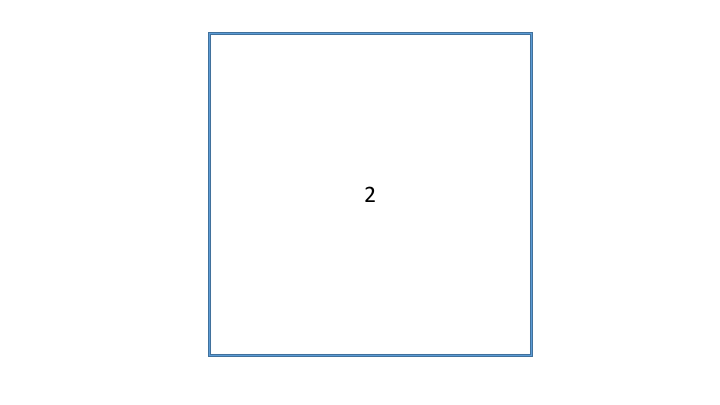
\includegraphics[width=1.5in, clip=true, trim=80mm 0mm 80mm 0mm]{figures/zone/Slide6.png}}
   \caption{Peers join and left CAN with self-merging enabled.}
   \label{fig:merging}
\end{figure} 

\begin{figure}[htbp] %  figure placement: here, top, bottom, or page
   \centering
   \subfigure[before peer3 left]{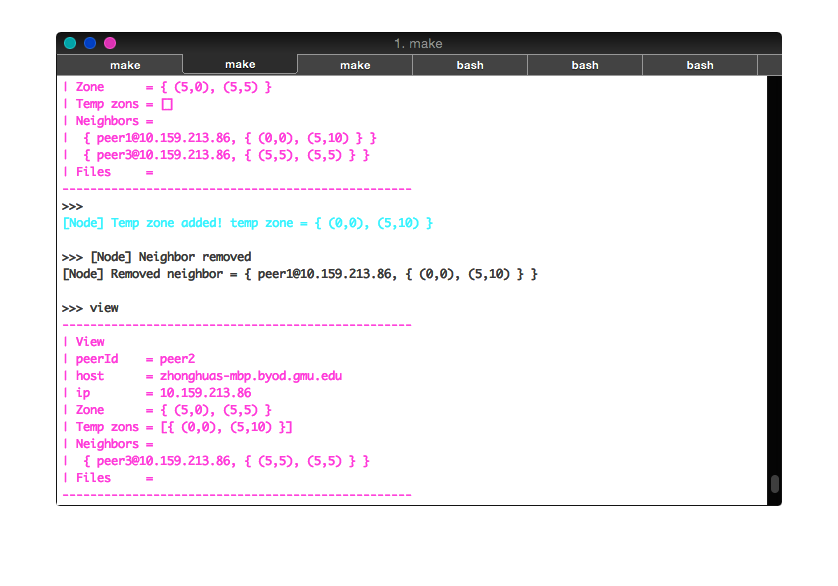
\includegraphics[width=5in, clip=true, trim=22mm 30mm 30mm 28mm]{figures/before.png}}
   \subfigure[after peer3 left]{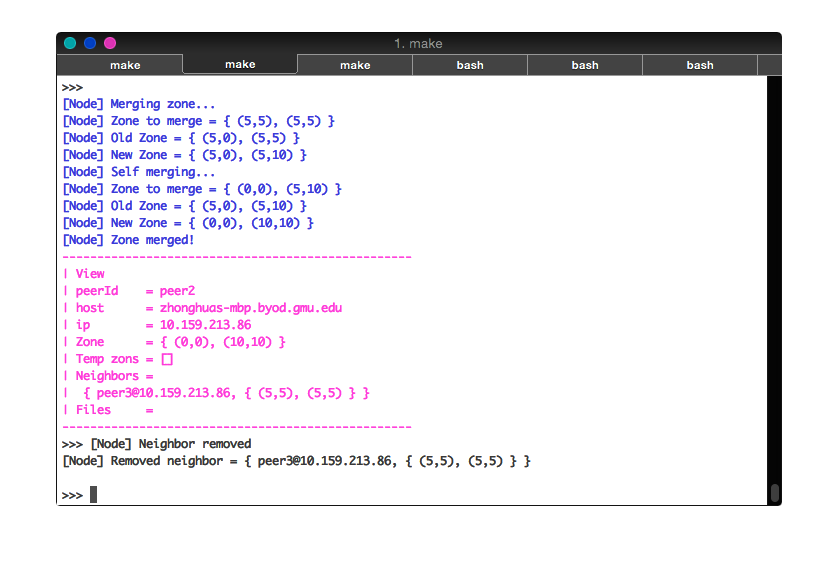
\includegraphics[width=5in, clip=true, trim=22mm 30mm 30mm 28mm]{figures/after.png}}
   \caption{Screenshots of self-merging process.}
   \label{fig:screenshot}
\end{figure} 

\subsection{File Insertion/Retrieval}
A file is inserted into CAN as a key value pair. Key is the keyword of the file, while the value is the content of the file. The following screenshots show the process of file insertion and retrieval on two nodes.

\begin{figure}[htbp] %  figure placement: here, top, bottom, or page
   \centering
      \subfigure[peer1]{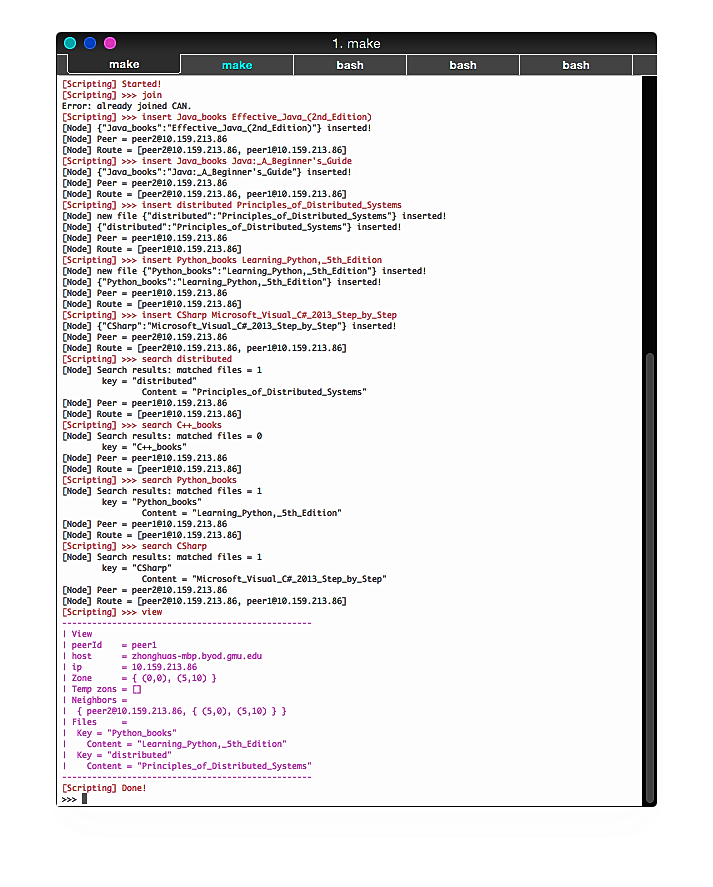
\includegraphics[width=2.9in, clip=true, trim=22mm 29mm 100mm 28mm]{figures/insertion2.png}}
   \subfigure[peer2]{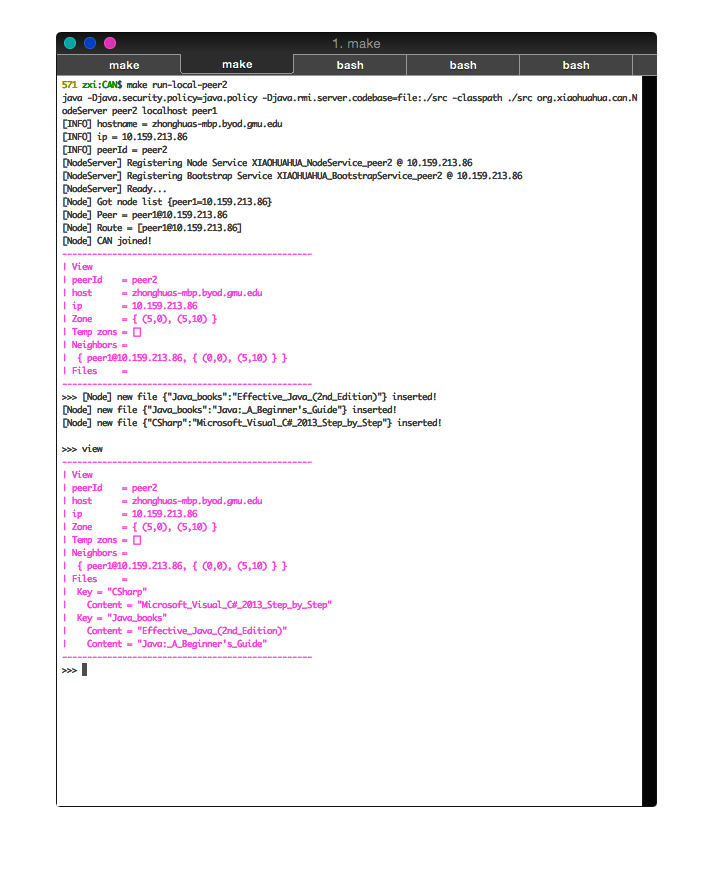
\includegraphics[width=2.9in, clip=true, trim=22mm 29mm 100mm 28mm]{figures/insertion1.png}}
   \caption{Screenshots of file insertion and retrivel.}
   \label{fig:insertion}
\end{figure} 

\end{document}  